\documentclass[12pt]{article}
\usepackage{amsmath}
\usepackage{amssymb}
\usepackage[letterpaper,margin=0.85in,centering]{geometry}
\usepackage{fancyhdr}
\usepackage{enumerate}
\usepackage{lastpage}
\usepackage{multicol}
\usepackage{graphicx}

\reversemarginpar

\pagestyle{fancy}
\cfoot{Page \thepage \ of \pageref{LastPage}}\rfoot{{\bf Total Points: 40}}
\chead{MATH 1010A}\lhead{Test \# 1}\rhead{Monday, 19\textsuperscript{th} October, 2015}

\newcommand{\points}[1]{\marginpar{\hspace{24pt}[#1]}}
\newcommand{\skipline}{\vspace{12pt}}
%\renewcommand{\headrulewidth}{0in}
\headheight 30pt

\newcommand{\di}{\displaystyle}
\newcommand{\R}{\mathbb{R}}
\newcommand{\aaa}{\mathbf{a}}
\newcommand{\bbb}{\mathbf{b}}
\newcommand{\ccc}{\mathbf{c}}
\newcommand{\dotp}{\boldsymbol{\cdot}}
\newcommand{\abs}[1]{\lvert #1\rvert}
\newcommand{\len}[1]{\lVert #1\rVert}
\newcommand{\ivec}{\,\boldsymbol{\hat{\imath}}}
\newcommand{\jvec}{\,\boldsymbol{\hat{\jmath}}}
\newcommand{\kvec}{\,\boldsymbol{\hat{k}}}
\DeclareMathOperator{\comp}{comp}

\begin{document}

\author{Instructor: Sean Fitzpatrick}
\thispagestyle{plain}
\begin{center}
\emph{University of Lethbridge}\\
Department of Mathematics and Computer Science\\
19\textsuperscript{th} October, 2015, 4:00 - 4:50 pm\\
{\bf MATH 1010A - Test \#1}\\
\end{center}
\skipline \skipline \skipline \noindent \skipline
Last Name:\underline{\hspace{353pt}}\\
\skipline
First Name:\underline{\hspace{350pt}}\\
\skipline
Student Number:\underline{\hspace{323pt}}\\
\skipline
Tutorial Section: \underline{\hspace{320pt}}\\


\vspace{0.5in}


\begin{quote}
 {\bf Record your answers below each question in the space provided.    Left-hand pages may be used as scrap paper for rough work.  If you want any work on the left-hand pages to be graded, please indicate so on the right-hand page.
 
 \bigskip
 
Partial credit will be awarded for partially correct work, so be sure to show your work, and include all necessary justifications needed to support your arguments.

\bigskip

No external aids are allowed, with the exception of a 5-function calculator.}
\end{quote}


\vspace{0.5in}

For grader's use only:

\begin{table}[hbt]
\begin{center}
\begin{tabular}{|l|r|} \hline
Page&Grade\\
\hline \hline
\cline{1-2} 2 & \enspace\enspace\enspace\enspace\enspace\enspace/10\\
\cline{1-2} 3 & \enspace\enspace\enspace\enspace\enspace\enspace/10\\
\cline{1-2} 4 & \enspace\enspace\enspace\enspace\enspace\enspace/10\\
\cline{1-2} 5 & \enspace\enspace\enspace\enspace\enspace\enspace/10\\
\cline{1-2} Total & \enspace\enspace\enspace\enspace\enspace\enspace/40\\
\hline
\end{tabular}

\skipline

\skipline

\skipline

B
\end{center}
\end{table}
\newpage


\begin{enumerate}
\item Simplify the following expressions. Your final answer should be in the form $\dfrac{A}{B}$, where $A$ and $B$ are integers.
\begin{enumerate}
 \item $\dfrac{1-\left(\frac{3}{5}\right)\left(\frac{5}{9}\right)}{1+\left(\frac{3}{5}\right)\left(\frac{5}{9}\right)}$. \points{3}

\vspace{1.75in}

 \item $\left(\dfrac{64}{125}\right)^{-2/3}$. \points{3}

\vspace{1.75in}

\end{enumerate}
\item Simplify the following expression. Your final answer should be in the form $\dfrac{A}{B}$, where $A$ and $B$ are polynomials.\points{4} 

\[
\di \frac{x+1}{2+x}+\frac{2x}{2-x}-\frac{5x+6}{4-x^2} 
\]

\newpage

\item Solve the following inequalities:
\begin{enumerate}
 \item $\dfrac{3}{4}-x \leq \dfrac{6x-2}{3}$. \points{3}

\vspace{2in}

 \item $5x\geq 2-x\geq 0$ \points{4}

\vspace{2in}

 \item $\lvert 2x+1\rvert <5$ \points{3}
\end{enumerate}
\newpage

\item Consider the function $f(x) = -x\lvert x\rvert$.
\begin{enumerate}
 \item Evaluate the following: $f(2), f(2) + f(-1), f(-2)\cdot f(3)$. \points{3}

\vspace{1.5in}

 \item Sketch the graph of $f$. (Hint: consider the cases $x\geq 0$ and $x<0$.) \points{3}

\begin{center}
 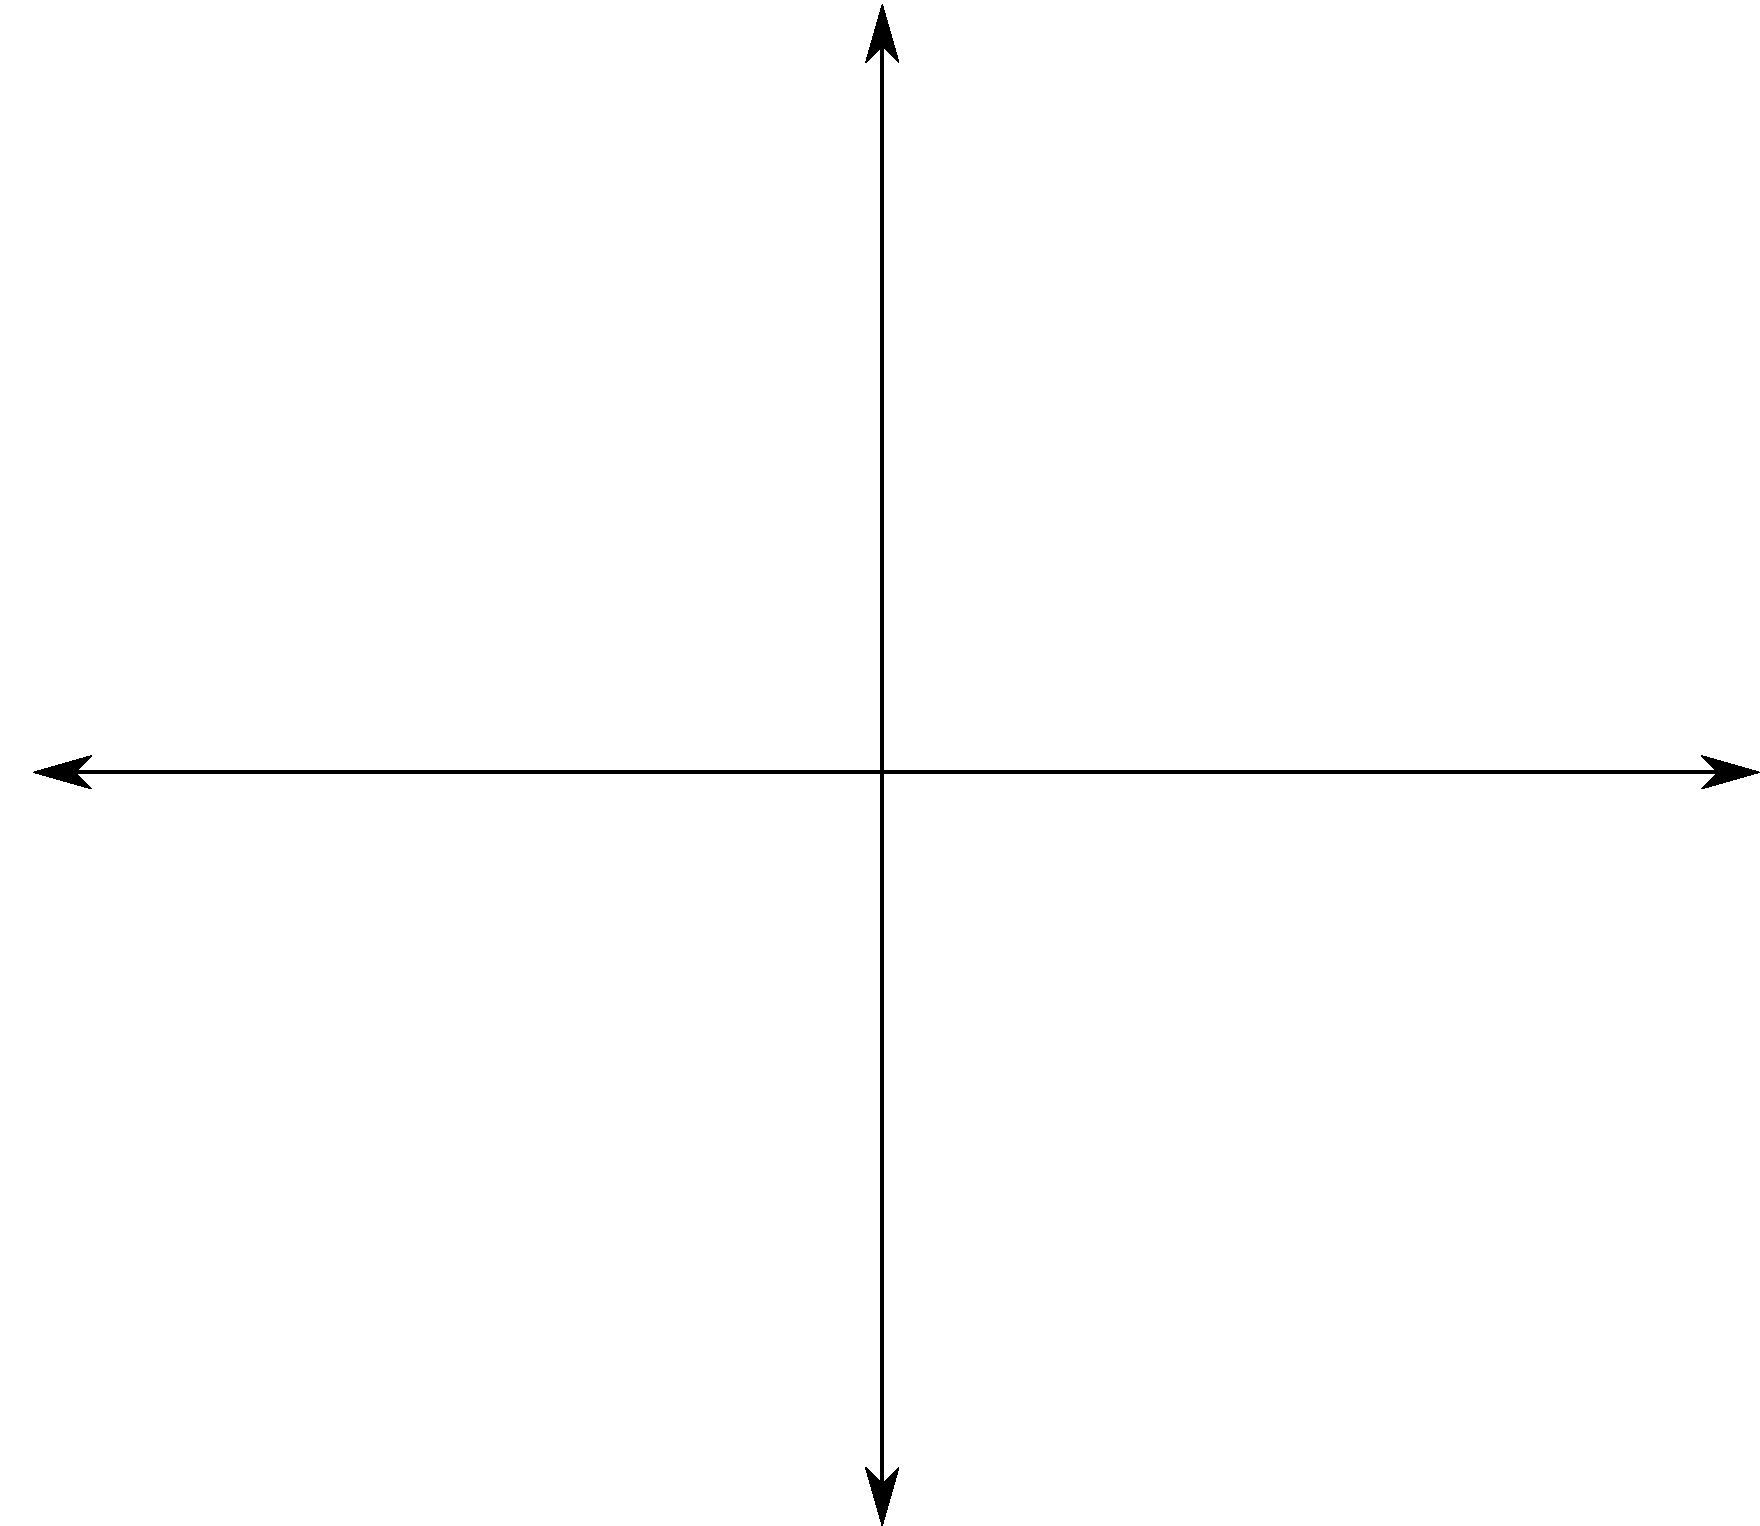
\includegraphics[height=2.5in]{axes.pdf}
\end{center}


 \item Sketch the graphs $y=f(x-3)$ and $y=-\frac{1}{3}f(x)+1$. \points{4}

{\bf Note:} if your graph in part (b) is incorrect, credit will be awarded for correct transformations of an incorrect graph.

\begin{multicols}{2}
 \begin{center}
 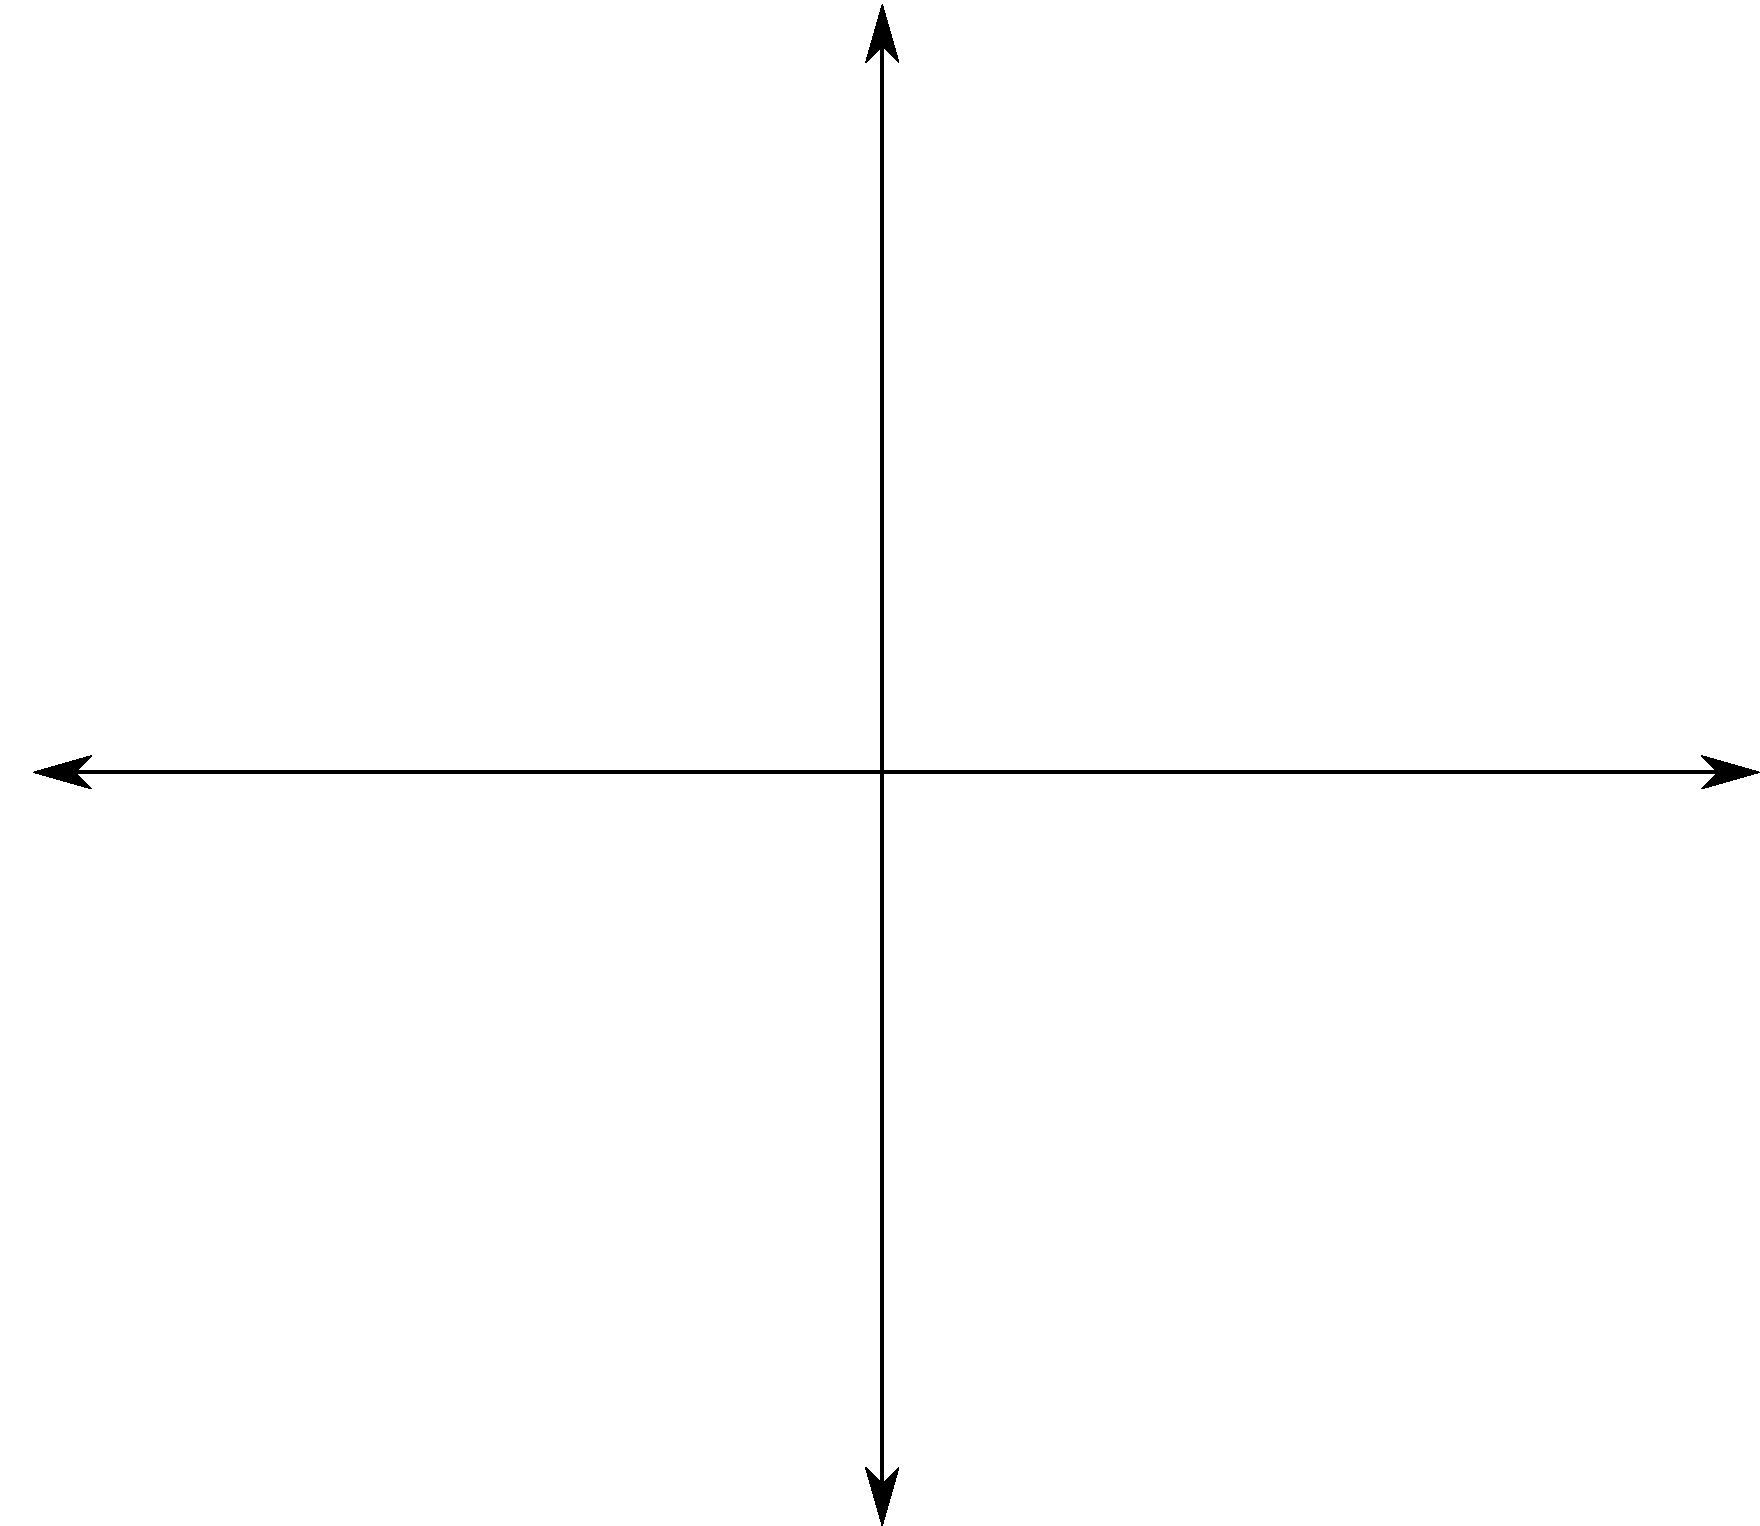
\includegraphics[height=2.5in]{axes.pdf}

$y=f(x-3)$
\end{center}
\begin{center}
 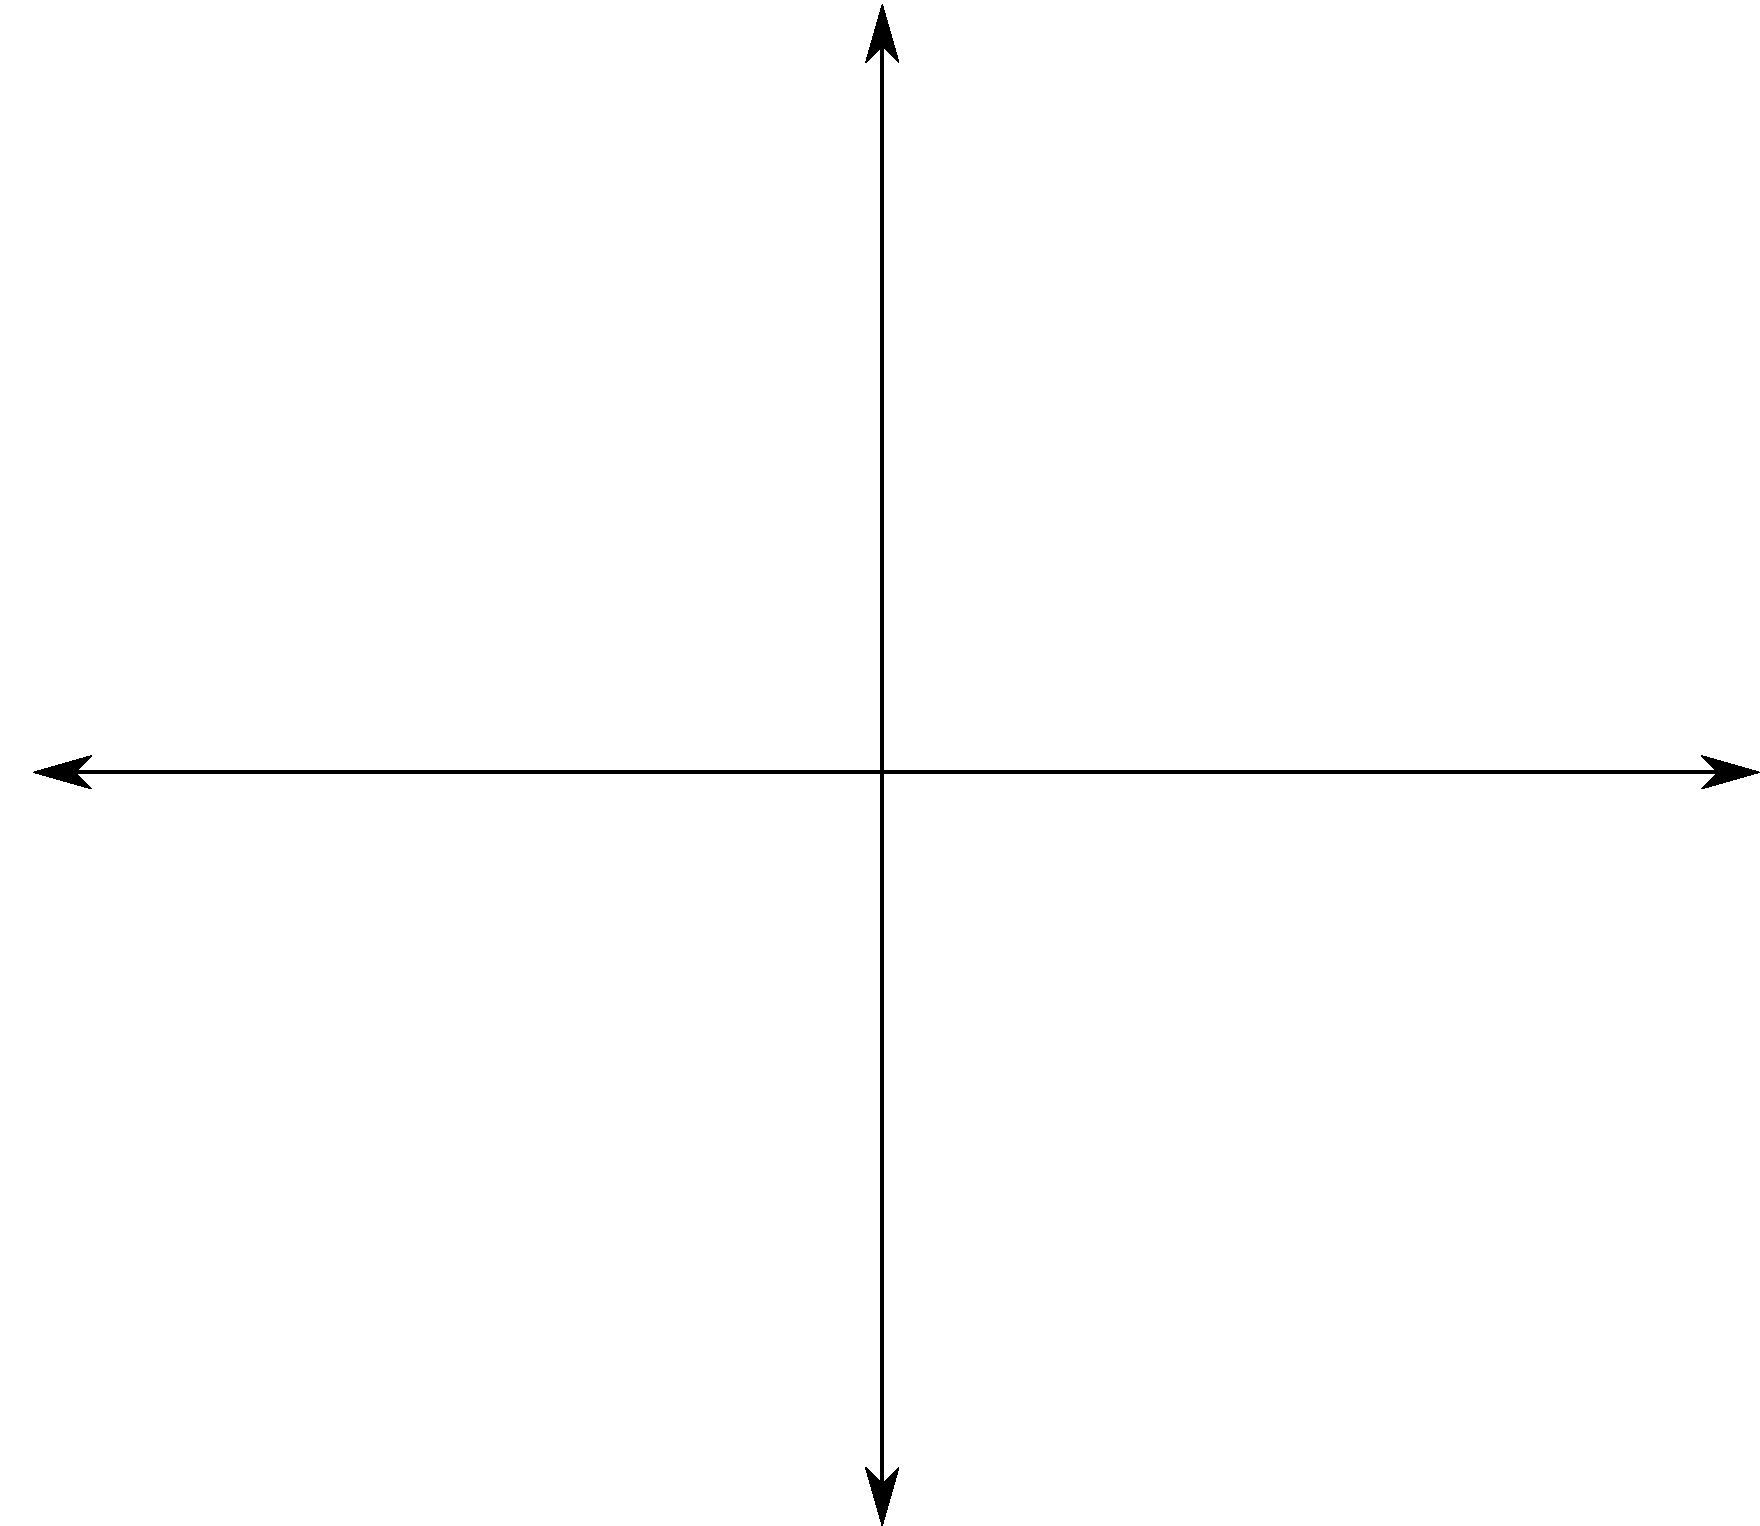
\includegraphics[height=2.5in]{axes.pdf}

$y=-\frac{1}{3}f(x)+1$
\end{center}
\end{multicols}

\end{enumerate}
\newpage

\item Consider the function $f(x) = x^2+4x-12$.
\begin{enumerate}
 \item Determine the sign diagram for $f$. \points{4}

\vspace{2in}

 \item Using your answer from part (a), solve the following:
\begin{enumerate}
 \item $f(x)=0$. \points{1}

\vspace{0.5in}

 \item $f(x)\geq 0$. \points{1}
\end{enumerate}

\vspace{0.75in}

\item Since $f$ is a quadratic function, its graph is a parabola. Determine the location of the vertex of the parabola, as well as any $x$ or $y$-intercepts. (You do not have to sketch the graph.) \points{3}

\vspace{2in}

\item What is the domain of the function $g(x) = \dfrac{1}{\sqrt{12-4x-x^2}}$? \points{1}



\end{enumerate}


\end{enumerate}
\end{document}